\begin{figure}
	\centering
	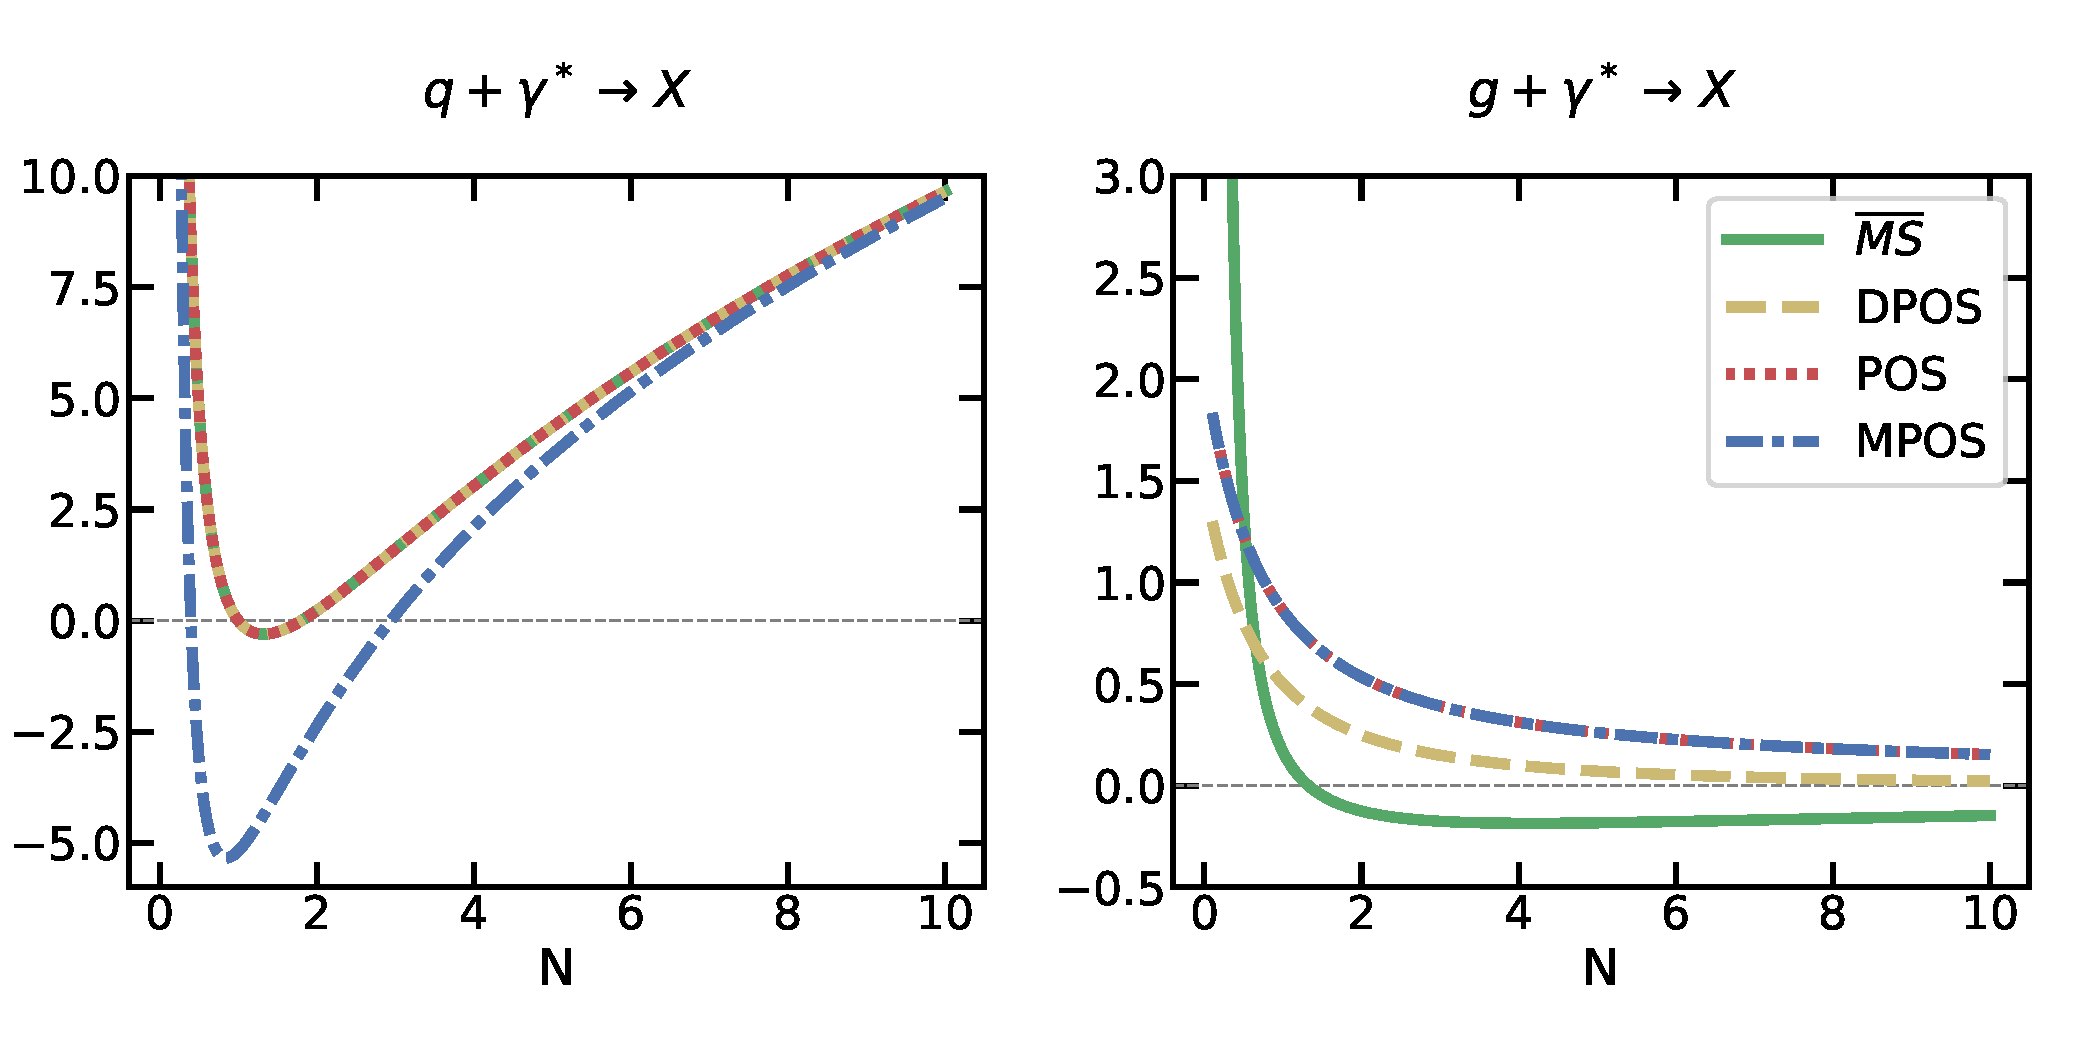
\includegraphics[width=0.7\textwidth]{ch-qcd/dis}
	\caption{The \acrfull{dis} process.}
	\label{fig:qcd/dis}
\end{figure}

\subsection{Kinematics}

The following kinematic variables are often used in the following:

\begin{align}
	Q^2   & = - q^2                       \\
	M_h^2 & = p^2                         \\
	\nu   & = q \cdot p                   \\
	x     & = \frac{Q^2}{2\nu}            \\
	y     & = \frac{q \cdot p}{k \cdot p}
\end{align}

so $M_h$ is the mass of the scattered hadron, while $x$ and
$y$ are Bjorken variables.

\paragraph{Hadronic vs Partonic} Notice that the variables listed here
are all \textbf{hadronic}, so $x$ is not the partonic momentum fraction (it is only
at \lo , because the coefficient function is a $\delta$).
In order to avoid confusion the coefficient function variable will be called
$z$, and thus the partonic momentum fraction will be $x/z$.

\begin{figure}
	\centering
	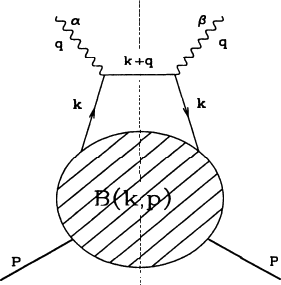
\includegraphics[width=0.4\hsize]{ch-yadism/handbag.png}
  \caption{The so-called \enquote{handbag} diagram.}
\end{figure}

The handbag diagram (B(k,p) are the \qcd corrections to the hadronic tensor)

So the hadronic tensor is given by

\begin{align}
      W_{\mu\nu} = \left(-g_{\mu\nu} + \frac{q_\mu q_\nu}{q^2}\right) F_1(x,Q^2)
                + \frac{\hat P_\mu \hat P_\nu}{P \cdot q} F_2(x,Q^2)
                \item i \varepsilon_{\mu\nu\alpha\beta} \frac{q^\alpha P^\beta}{2 P\cdot q} F_3(x,Q^2)
\end{align}

with $\hat P_\mu = P_\mu - (P\cdot q / q^2) q_\mu$, $P$ the 4-momentum of the
hadron and $q$ the 4-momentum of the scattered boson.

\subsection{Process / Currents}

\texttt{yadism} allows to compute three different type of \textbf{processes}, which correspond to a
given set of scattering bosons:

\begin{itemize}
  \item \acrfull{ec}: we only allow the photon to be exchanged.
    This is the most basic setup and in many cases the only allowed option.
  \item \acrfull{nc}: in addition to the photon we also allow for the
    $Z$ boson to be exchanged, so this is a superset of \ec.
    Since now two bosons are allowed also interference terms appear.
    The $Z$ boson has an axial coupling to the leptons and thus it introduces the
    problems related to $\gamma_5$ \cite{Gnendiger:2017pys}.
    Note that there are no Flavor Changing Neutral Currents (FCNC) in the \sm,
    but they are an active field of research.
  \item \acrfull{cc}: we only allow the $W^+$ \textit{or} $W^-$ to be
    exchanged. The actual boson is determined by the incoming scattering lepton
    and charge conservation. As the $W^\pm$ are flavor changing additional care
    is needed in the calculation.
\end{itemize}


\subsection{Structure Function Kind}

\texttt{yadism} allows to compute three different structure functions, to which we refer to as \textbf{kind}:

\begin{align}
    F_2,~ F_L = F_2 - 2xF_1,~ xF_3
\end{align}

\begin{itemize}
\item to compute $F_L$ instead of $F_1$ is adventagous due to the Callan-Gross relation
  \cite{Callan:1969uq} $F_L=0$ in the naive parton model
  \begin{itemize}
  \item notice that the $F_L$ definition it's not exactly the one above, but
    it may be corrected (actually $F_L$ it's the object involved in
    Callan-Gross relation, for more information see :ref:`fl-corrections`)
  \end{itemize}
\item Note that we compute $xF_3$ instead of the bare structure function to respect the native
  scaling in the full cross section
\end{itemize}
Even $F_1$ is provided, but it is treated as a derived quantity, like the cross
sections in the following section.
